\section{User Interface}
When the program is opened for the first time, there are already default vertex and fragment shaders, and a "default material". This is a simple material that will be assigned to new objects upon creation. For the common use case, this material can be ignored.

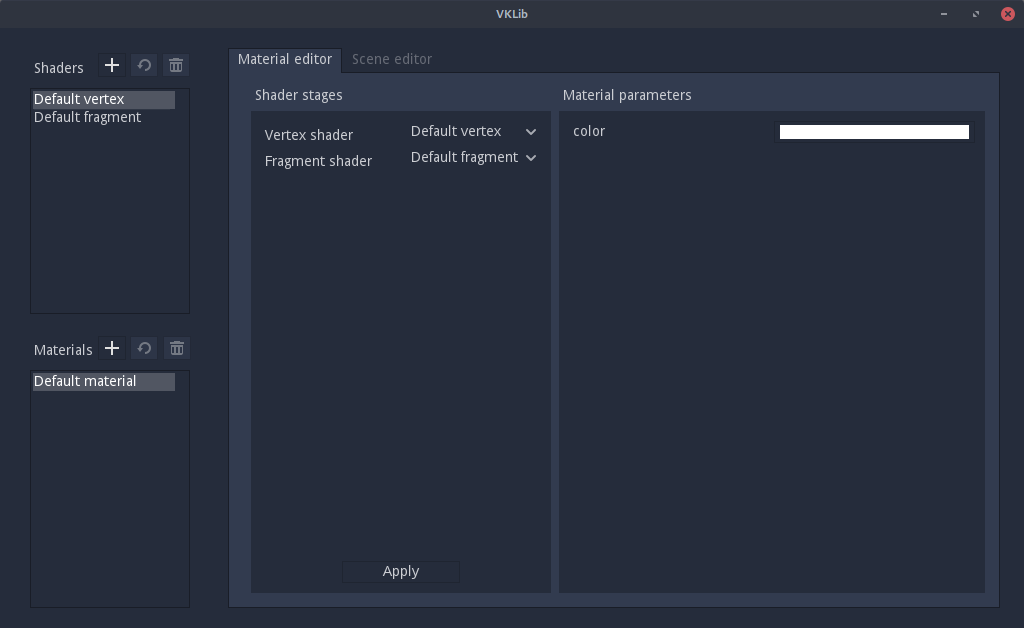
\includegraphics{01-control}

The user will program the shader using their favorite editor of choice, in GLSL. The shaders' source code must be saved in separate files, ending in ".vert" for the vertex shader and ".frag" for the fragment shader. Then, using our application, the user will load each of these files as a new shader, and give it a name (the shader name defaults to the file name and must be unique). If the shader compilation fails, the shader will not be created, and the compilation error message is displayed in the console. Having created both vertex and fragment shaders successfully, the user can then create a new material and give it a name, which also has to be unique. After the material is created, clicking on it will reveal a panel where the user can change the shaders used in the material. On newly created materials, the default shaders will be used. After choosing the shaders from the drop-down menus, the "apply" button will update the material with the new shaders, and the uniforms defined in the shaders will appear in the editor on the rightmost panel, ready to be modified.

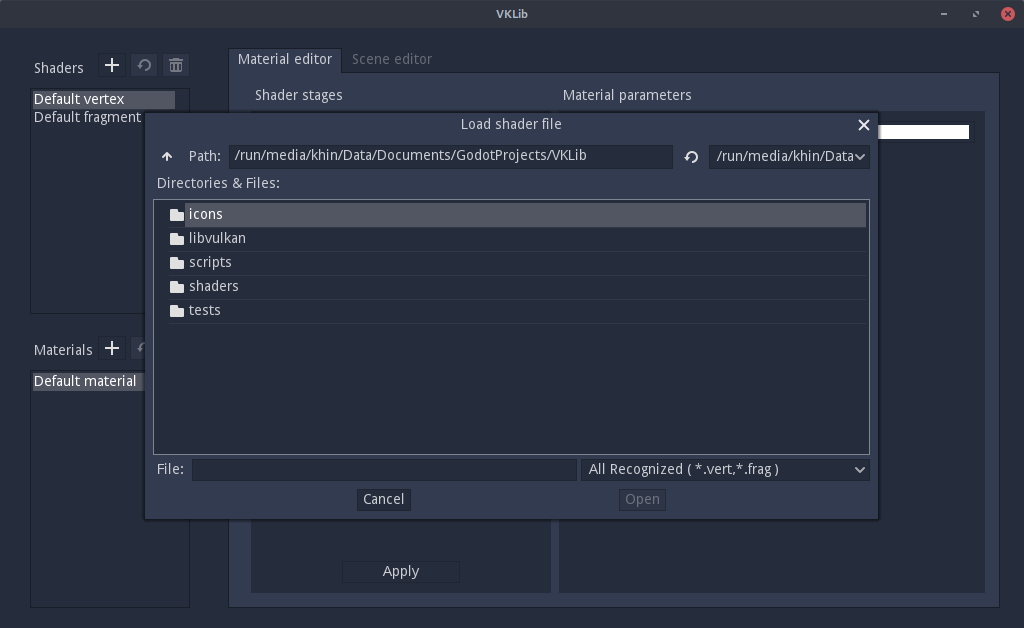
\includegraphics{02-load shader}

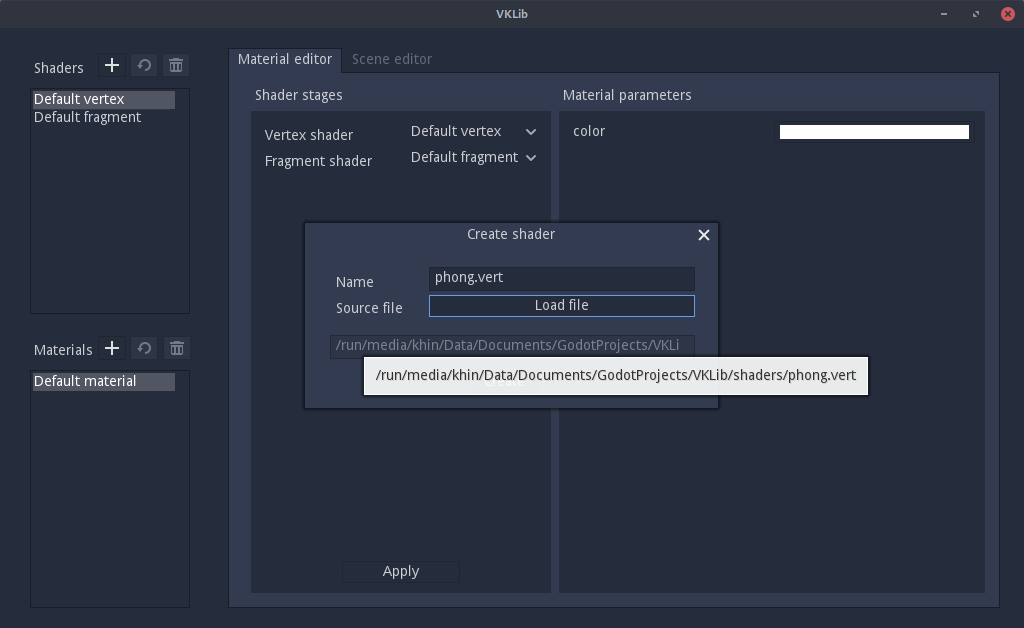
\includegraphics{03-create shader}

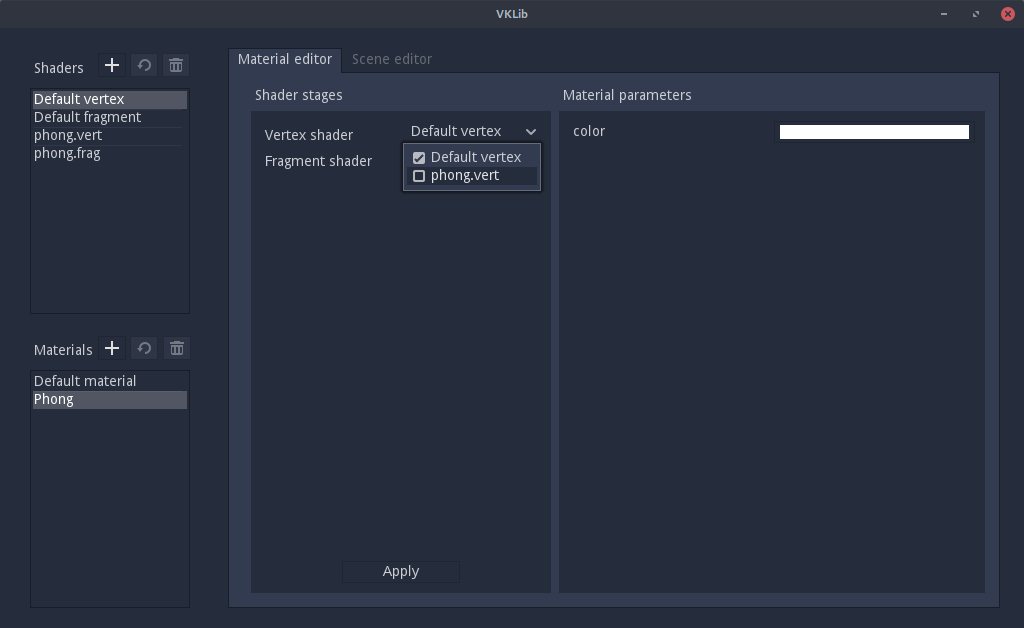
\includegraphics{04-material edit}

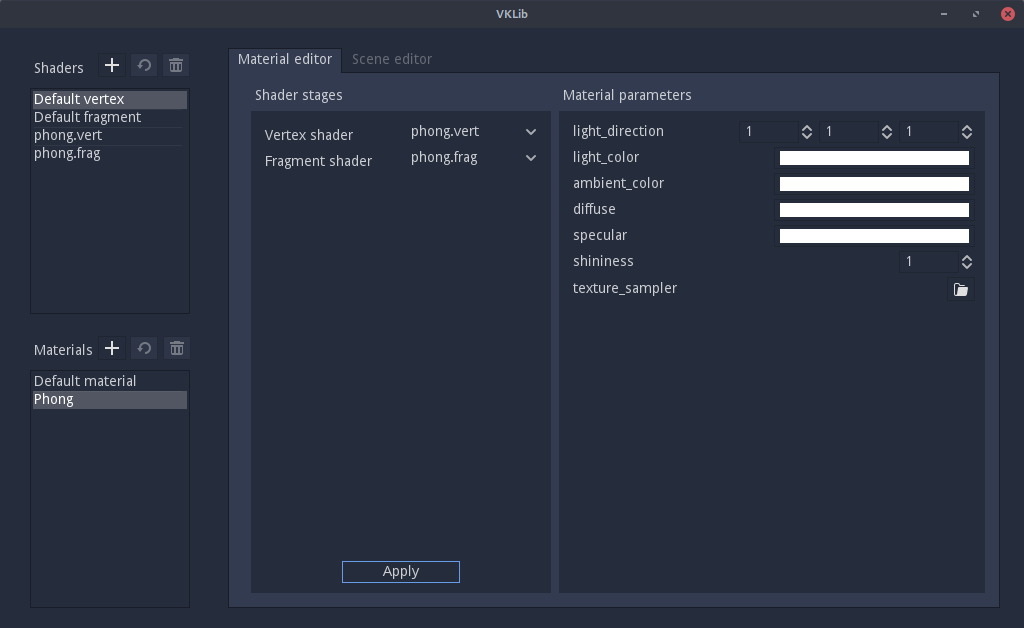
\includegraphics{05-uniforms}

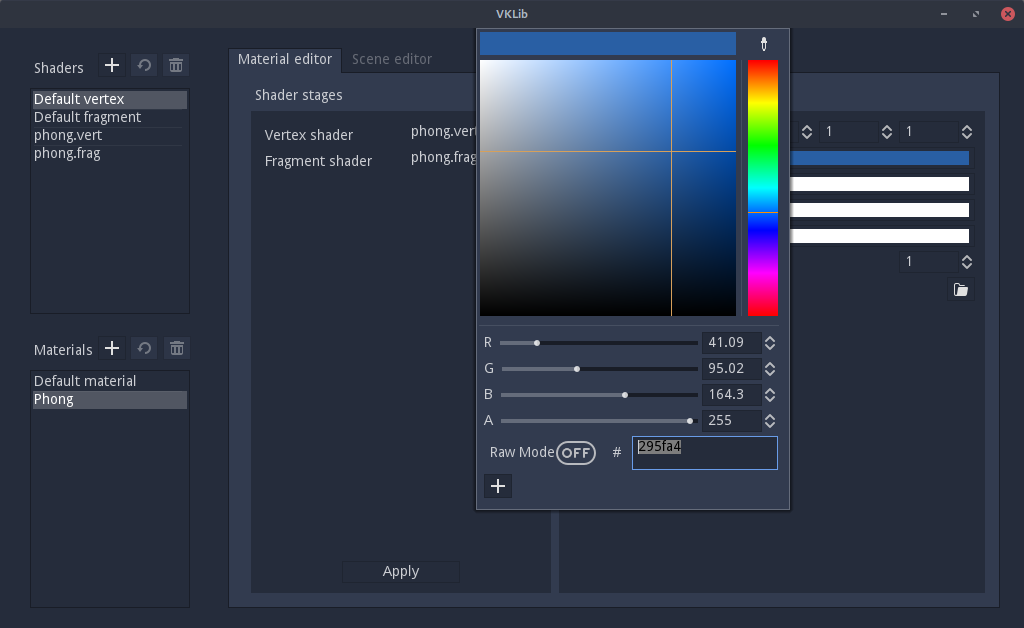
\includegraphics{06-uniform edit}

Objects can be created in the "Scene Editor" tab. Currently, only geometric primitives can be created, like cubes, spheres, capsules and planes (rather than loading custom objects). Objects are given a name based on their shape (the geometry itself) and their creation order. When an object is selected from the list, their transform is exposed in the rightmost panel, so the user can change the object's position, rotation and scale, and also the material used to render it. When first created, the default material will be used.

% include prints of the scene editor

Once the object is created, it should appear in the Vulkan visualization window. To move the camera, the user can right-click inside the window to enter movement mode, an use the WASD keys to move around, Q to move down and E to move up. Moving the mouse will turn the camera in a free-look style.
